\documentclass[10pt,a4paper]{article}

% ---------- Packages ----------
\usepackage[T1]{fontenc}
\usepackage[utf8]{inputenc}
\usepackage{lmodern}
\usepackage[top=0.9in,bottom=0.9in,left=0.9in,right=0.9in,headheight=14pt]{geometry}
\usepackage{amsmath,amssymb}
\usepackage{microtype}
\usepackage{booktabs}
\usepackage{array}
\usepackage{enumitem}
\usepackage{listings}
\usepackage{fancyhdr}
\usepackage{titlesec}
\usepackage{graphicx}
\usepackage{caption}
\usepackage{setspace}
\usepackage{tikz}
\usetikzlibrary{shapes.geometric, arrows.meta, positioning}
\usepackage[hidelinks]{hyperref}

% ---------- Global style (black and white only) ----------
\setlength{\parindent}{0pt}
\setlength{\parskip}{4pt}
\setlist{itemsep=2pt,topsep=3pt}
\renewcommand{\arraystretch}{1.2}
\setstretch{1.0}
\captionsetup{font=small,labelfont=bf,labelsep=period}

\pagestyle{fancy}
\fancyhf{}
\fancyhead[L]{\small\itshape Large-Scale Job Market Intelligence and Emerging Skill Demand Analysis}
\fancyhead[R]{\small\itshape CSE412 Final Project Report}
\fancyfoot[C]{\small\thepage}
\renewcommand{\headrulewidth}{0.4pt}
\fancypagestyle{plain}{\fancyhf{}\fancyfoot[C]{\small\thepage}\renewcommand{\headrulewidth}{0pt}}

\titleformat{\subsection}{\normalfont\Large\bfseries}{\thesection}{0.6em}{}
\titlespacing*{\subsection}{0pt}{12pt}{4pt}
\titleformat{\subsubsection}{\normalfont\large\bfseries}{\thesubsection}{0.6em}{}
\titlespacing*{\subsubsection}{0pt}{8pt}{3pt}
\titleformat{\subsubsection}{\normalfont\normalsize\bfseries\itshape}{\thesubsubsection}{0.6em}{}
\titlespacing*{\subsubsection}{0pt}{6pt}{2pt}

\lstset{
  basicstyle=\ttfamily\small,
  frame=single,
  breaklines=true,
  columns=fullflexible,
  xleftmargin=4pt, xrightmargin=4pt,
  aboveskip=8pt, belowskip=8pt
}

\newcommand{\code}[1]{\texttt{\small\detokenize{#1}}}
\newcommand{\rupee}{INR~}

\begin{document}

% =====================================================
%                    TITLE PAGE
% =====================================================
\begin{titlepage}
\thispagestyle{empty}
\centering
\vspace*{1cm}
{\large\bfseries INDIAN INSTITUTE OF INFORMATION TECHNOLOGY KOTTAYAM\par}
\vspace{0.4cm}
{\normalsize Department of Computer Science and Engineering\par}
\vspace{1.5cm}
\rule{\textwidth}{1.2pt}\par
\vspace{0.6cm}
{\Huge\bfseries Large-Scale Job Market Intelligence\\and Emerging Skill Demand Analysis\par}
\vspace{0.6cm}
{\Large An End-to-End Big Data Architecture\\Using HDFS, Apache Pig, and Apache Hive\par}
\vspace{0.6cm}
\rule{\textwidth}{1.2pt}\par
\vspace{1.5cm}
{\large\bfseries Final Project Report\par}
\vspace{0.3cm}
{\large CSE412 --- Big Data \& Large-Scale Computing\par}
\vspace{1.8cm}

{\large\bfseries Submitted by\par}
\vspace{0.4cm}
\begin{tabular}{lr}
N Medhashree & 2023BCS0042 \\
Ashmi S N & 2023BCS0196 \\
Deepanjali Tudu & 2023BCS0066 \\
\end{tabular}

\vspace{1.5cm}
{\normalsize\textbf{Repository:} \url{https://github.com/medhashree05/JOB_MARKET_ANALYSIS}\par}
\vspace{0.3cm}

\vfill
\end{titlepage}


% =====================================================
%                    ABSTRACT
% =====================================================
\section*{Abstract}
\addcontentsline{toc}{section}{Abstract}

Modern online recruitment portals publish tens of thousands of unstructured, heterogeneous job postings weekly. Extracting actionable labour-market intelligence from this corpus requires scalable, fault-tolerant batch architectures capable of handling noisy free text, multi-valued skill lists, inconsistent geographic spellings, and non-standard salary disclosures. This project designs, implements, and empirically verifies an end-to-end Big Data processing pipeline over a primary dataset of 97,929 Indian job postings.

The pipeline integrates three core Hadoop ecosystem layers: (1)~\textbf{HDFS ingestion and sanitisation}, which performs deterministic schema validation and deduplication, retaining 97,679 verified postings; (2)~\textbf{Apache Pig}, which performs parallel tokenisation, normalisation, distinct job--skill projection, and multi-dimensional aggregation on MapReduce; and (3)~\textbf{Apache Hive}, which exposes the aggregated partitions as structured external tables via \code{OpenCSVSerde} and evaluates analytical HiveQL queries across job roles, skills, hiring hubs, and salary benchmarks. A decoupled \textbf{Streamlit presentation layer} provides an interactive seven-page dashboard with CSV export.

A technical audit of the repository resolved earlier numerical discrepancies: the variances between 97,679 and 97,715 postings, and between 18,320 and 18,310 Bengaluru postings, are traced to a 36-row newline fragmentation artifact in unquoted intermediate CSV exports. Because the primary dataset is a cross-sectional scrape with relative recency strings rather than multi-year calendar dates, temporal trend measurement is structurally constrained. The \textbf{Skill Demand Velocity Index (SDVI)} is therefore evaluated as a conceptual extension, and a mathematical audit shows the limitations of single-scalar quadrant thresholding and proposes an orthogonal two-dimensional classification.

\vspace{0.5cm}
\textbf{Keywords:} Big Data, HDFS, Apache Pig, Apache Hive, MapReduce, Job Market Analytics, Skill Demand, Streamlit.

\vspace{0.5cm}
\tableofcontents
\newpage


% =====================================================
%                 1. INTRODUCTION
% =====================================================
\section{Introduction}

\subsection{Background and Motivation}
Labour-market intelligence provides critical signals for curriculum planning, workforce development, and industrial hiring strategy. However, large-scale recruitment data is notoriously noisy: identical job titles appear with arbitrary capitalisation and parenthetical annotations; skill requirements are packed into single comma-delimited strings; salary disclosures are sparse, right-skewed, and multi-currency; and posting dates frequently rely on relative timestamps (e.g., ``3 Days Ago'') without an absolute scrape reference. Processing such corpora at scale exceeds the capabilities of in-memory single-node spreadsheets and calls for a distributed, fault-tolerant Big Data architecture.

\subsection{Objectives}
This project delivers a complete, reproducible batch-processing pipeline for large-scale job market intelligence, organised into four layers:
\begin{itemize}
  \item \textbf{Storage Layer (HDFS):} distributed ingestion, block-level storage, replication, and data validation.
  \item \textbf{Transformation Layer (Apache Pig):} procedural MapReduce dataflows for schema enforcement, string parsing, skill-array flattening, and grouped aggregations.
  \item \textbf{Analytical Warehouse (Apache Hive):} schema-on-read external tables, \code{OpenCSVSerde} parsing for text preservation, and HiveQL analytical querying.
  \item \textbf{Exploration Layer (Streamlit and Plotly):} a decoupled presentation dashboard delivering executive KPIs, geographic drill-downs, and filtered data exploration.
\end{itemize}

\subsection{Scope and Empirical Boundaries}
The primary empirical pipeline is verified over the \textbf{Indian Job Market Dataset 2025} (97,929 raw records). All reported metrics for role demand, skill popularity, geographic hiring distribution, and disclosed compensation are computed from verified execution artifacts on Hadoop 3.3.6 and Hive 3.1.3.

The report distinguishes between verified empirical work and conceptual extensions:
\begin{enumerate}[label=(\alph*)]
  \item \textbf{Verified Empirical Pipeline (Phase~I):} full ingestion, cleaning, MapReduce execution in Pig, Hive table materialisation, and interactive dashboard analytics over 97,679 verified postings.
  \item \textbf{Conceptual Velocity Framework (Phase~II, SDVI):} a theoretical framework for measuring longitudinal skill momentum across dated postings, accompanied by a mathematical critique of its quadrant boundary conditions.
\end{enumerate}

\subsection{Report Organisation}
Section~2 reviews related literature. Section~3 describes the system architecture and execution environment. Section~4 details the implementation of each pipeline stage. Section~5 reconciles numerical discrepancies. Section~6 presents the verified empirical findings. Section~7 describes the dashboard. Section~8 audits the Phase~II SDVI framework. Section~9 discusses data-quality limitations, and Section~10 concludes with future work.

% =====================================================
%                 2. LITERATURE REVIEW
% =====================================================
\section{Literature Review}

\subsection{Distributed Batch Computing Foundations}
The foundation of large-scale distributed computing was formulated by Dean and Ghemawat~\cite{dean2004mapreduce}, who introduced the MapReduce programming paradigm to parallelise computation across commodity clusters with automatic data partitioning, scheduling, and fault recovery. The underlying storage fabric, the Hadoop Distributed File System (HDFS), described by Shvachko et al.~\cite{shvachko2010hdfs}, provides high-throughput streaming access to large files via block-level distribution across DataNodes coordinated by a centralised NameNode metadata service.

\subsection{High-Level Dataflow and Warehousing Abstractions}
Writing native MapReduce in Java involves substantial boilerplate and complex join and aggregation management. To abstract this complexity, Olston et al.~\cite{olston2008pig} developed Pig Latin, a procedural dataflow language that compiles high-level transformations (\code{FILTER}, \code{FOREACH}, \code{GROUP}, \code{COGROUP}, \code{FLATTEN}) into directed acyclic graphs of MapReduce jobs. Concurrently, Thusoo et al.~\cite{thusoo2009hive} introduced Apache Hive, establishing the schema-on-read warehousing model. Hive projects SQL-like structures (HiveQL) over distributed files and supports metadata separation, partition pruning, and serialisers/deserialisers such as \code{OpenCSVSerde}. White~\cite{white2015hadoop} provides comprehensive guidance on integrating HDFS, Pig, and Hive in production clusters.

\subsection{Skill Extraction and Labour-Market Analytics}
Analysing online recruitment advertisements has become an important discipline in computational economics. Khaouja et al.~\cite{khaouja2021survey} surveyed text-mining and natural language processing approaches for skill extraction, noting that while machine-learning taggers offer high specificity, distributed rule-based tokenisation remains well suited to high-throughput batch pipelines. Djumalieva and Sleeman~\cite{djumalieva2018taxonomy} demonstrated that data-driven skill taxonomies derived from online vacancy text can track emerging industry requirements before formal occupation classification systems (such as O*NET or SOC) are updated.

\subsection{Momentum Metrics and Percentage Distortion}
In longitudinal skill analysis, ranking by raw frequency introduces \textit{incumbent inertia}: foundational skills such as SQL and Python dominate total counts regardless of current market acceleration. Conversely, naive percentage growth suffers from \textit{sparsity distortion}: a tool growing from 1 to 3 postings shows $+200\%$ growth, overshadowing an enterprise tool growing from 500 to 750 postings ($+50\%$). Weighting growth by logarithmic volume, as conceptualised in velocity metrics, addresses both pitfalls.

% =====================================================
%                 3. SYSTEM DESIGN
% =====================================================
\section{System Architecture and Environment}

\subsection{End-to-End Architecture}
The pipeline follows a decoupled, staged architecture designed for linear horizontal scalability. Figure~\ref{fig:architecture} illustrates the dataflow from raw ingestion through distributed transformation to presentation.

\begin{figure}[htbp]
\centering
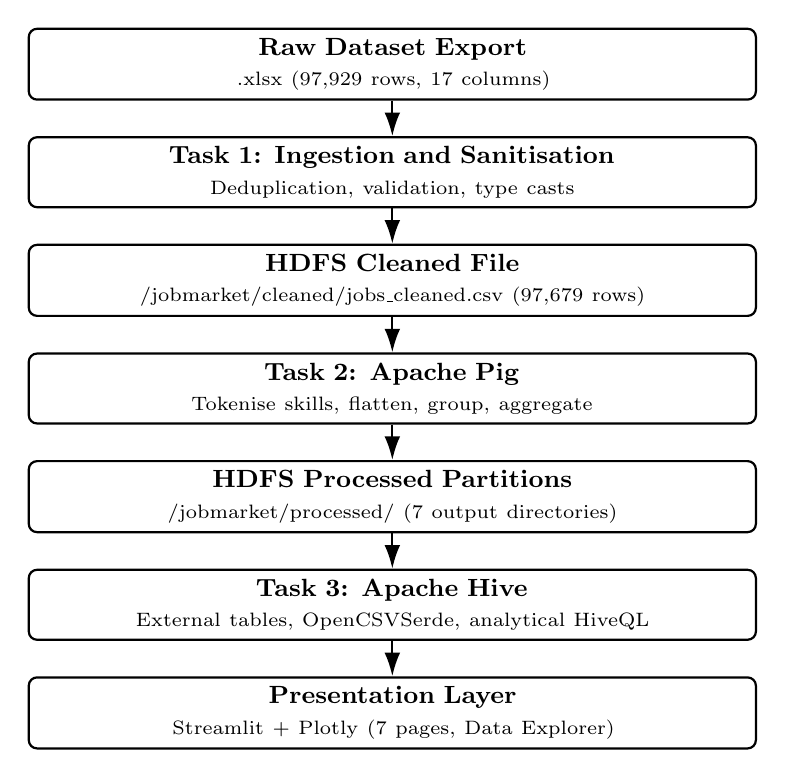
\begin{tikzpicture}[
  node distance=0.45cm,
  block/.style={rectangle, draw=black, thick, rounded corners=3pt, text width=9cm, minimum height=0.8cm, align=center, font=\small},
  arrow/.style={-{Latex[length=3mm, width=2mm]}, thick}
]
  \node[block] (raw) {\textbf{Raw Dataset Export}\\{\scriptsize .xlsx (97,929 rows, 17 columns)}};
  \node[block, below=of raw] (t1) {\textbf{Task 1: Ingestion and Sanitisation}\\{\scriptsize Deduplication, validation, type casts}};
  \node[block, below=of t1] (hdfs_clean) {\textbf{HDFS Cleaned File}\\{\scriptsize /jobmarket/cleaned/jobs\_cleaned.csv (97,679 rows)}};
  \node[block, below=of hdfs_clean] (t2) {\textbf{Task 2: Apache Pig}\\{\scriptsize Tokenise skills, flatten, group, aggregate}};
  \node[block, below=of t2] (hdfs_proc) {\textbf{HDFS Processed Partitions}\\{\scriptsize /jobmarket/processed/ (7 output directories)}};
  \node[block, below=of hdfs_proc] (t3) {\textbf{Task 3: Apache Hive}\\{\scriptsize External tables, OpenCSVSerde, analytical HiveQL}};
  \node[block, below=of t3] (dash) {\textbf{Presentation Layer}\\{\scriptsize Streamlit + Plotly (7 pages, Data Explorer)}};

  \draw[arrow] (raw) -- (t1);
  \draw[arrow] (t1) -- (hdfs_clean);
  \draw[arrow] (hdfs_clean) -- (t2);
  \draw[arrow] (t2) -- (hdfs_proc);
  \draw[arrow] (hdfs_proc) -- (t3);
  \draw[arrow] (t3) -- (dash);
\end{tikzpicture}
\caption{End-to-end Big Data pipeline across HDFS, Apache Pig, Apache Hive, and Streamlit.}
\label{fig:architecture}
\end{figure}

\subsection{Cluster Execution Environment}
All pipeline stages were executed and verified on a dedicated Big Data lab environment hosted on WSL~2 (Ubuntu 22.04 LTS), as summarised in Table~\ref{tab:env}.

\begin{table}[htbp]
\centering
\small
\begin{tabular}{@{}p{3.6cm}p{4.2cm}p{6.2cm}@{}}
\toprule
\textbf{Component} & \textbf{Version} & \textbf{Configuration and Path} \\
\midrule
Operating System & Ubuntu 22.04 LTS (WSL 2) & Linux kernel 5.15.167.4-microsoft-standard-WSL2 \\
Java Development Kit & OpenJDK 1.8.0\_422 & \code{/usr/lib/jvm/java-8-openjdk-amd64} \\
Distributed File System & Apache Hadoop 3.3.6 & \code{/usr/local/hadoop} (replication factor 1) \\
MapReduce Processing & Apache Pig 0.17.0 & \code{/usr/local/pig} (Piggybank enabled) \\
Data Warehouse & Apache Hive 3.1.3 & \code{/usr/local/hive} (database \code{jobmarket}) \\
Presentation Runtime & Python 3.13, Streamlit 1.39 & local virtual environment (\code{dashboard/.venv}) \\
\bottomrule
\end{tabular}
\caption{Software stack and execution environment.}
\label{tab:env}
\end{table}

% =====================================================
%                 4. IMPLEMENTATION
% =====================================================
\section{Pipeline Implementation}

\subsection{Task 1: Ingestion, Sanitisation, and Schema Contract}
The raw dataset (\code{indian-job-market-dataset-2025.xlsx}) contains 97,929 recruitment postings. Ingestion and data hygiene are implemented in Python (\code{01_convert_xlsx_to_csv.py} and \code{02_clean_data.py}):
\begin{enumerate}
  \item \textbf{Deduplication:} 247 exact duplicate rows were detected and removed. A subset deduplication on \code{job_id} removed 3 additional records, eliminating exactly \textbf{250 duplicate rows}.
  \item \textbf{Schema validation:} mandatory constraints were asserted on primary identifiers: $\text{job\_id} \neq \emptyset$, $\text{job\_title} \neq \emptyset$, and $\text{location\_raw} \neq \emptyset$. All 97,679 unique records satisfied required-field completeness.
  \item \textbf{Salary normalisation:} in the raw scrape, 64,076 postings lacked compensation figures, labelled \code{"Not disclosed"} with minimum and maximum salary hard-coded to \code{0.0}. To prevent downward bias, these values were converted to \code{NaN} (missing). Postings explicitly labelled \code{"Unpaid"} (333 records) retained \code{0.0} as a valid compensation value.
  \item \textbf{Primary location extraction:} multi-location strings (e.g., \code{"Kolkata(Chinar Park)"} or \code{"Noida, Greater Noida"}) were parsed to isolate the primary municipal hiring centre (\code{"Kolkata"}, \code{"Noida"}) while retaining \code{location_raw} for auditing.
  \item \textbf{Sanitised retention:} the validated dataset retains exactly \textbf{97,679 records} (99.74\% retention) and is staged to HDFS at \code{/jobmarket/cleaned/jobs_cleaned.csv}.
\end{enumerate}

\subsection{Task 2: Transformation Using Apache Pig}
The script \code{task2_jobmarket.pig} loads the cleaned CSV from HDFS using Piggybank's \code{CSVExcelStorage(',')}, drops the header row, and executes five core transformations:
\begin{itemize}
  \item \textbf{Case and whitespace normalisation:} applies \code{LOWER(TRIM())} to titles and locations.
  \item \textbf{Skill array explosion:} evaluates \code{FLATTEN(TOKENIZE(skills, ','))}, strips whitespace, purges null and \code{"not specified"} tokens, and enforces \code{DISTINCT} on \code{(job_id, skill)} pairs so that no posting counts twice for the same skill.
  \item \textbf{Multi-dimensional grouping:} aggregates posting volume by skill, by primary location, and by job role.
  \item \textbf{Currency separation:} computes minimum, maximum, and mean salary by role and by location, filtering $\text{avg\_salary} > 0$ and partitioning INR and USD into non-overlapping groups.
  \item \textbf{Recency binning:} groups relative posting strings into recency categories (\code{0-1 Days}, \code{1-7 Days}, \code{7-30 Days}, \code{30+ Days}, \code{Unknown}).
\end{itemize}

All seven output directories were written to HDFS with completed part files (Table~\ref{tab:hdfs}).

\begin{table}[htbp]
\centering
\small
\begin{tabular}{@{}p{4.3cm}p{5.2cm}p{2.2cm}r@{}}
\toprule
\textbf{HDFS Output Path} & \textbf{Content} & \textbf{Part File} & \textbf{Size} \\
\midrule
\code{/jobmarket/processed/jobs} & Normalised master job records & \code{part-m-00000} & 24.25 MB \\
\code{/jobmarket/processed/skills} & Unique (job\_id, skill) pairs & \code{part-r-00000} & 53.36 MB \\
\code{/jobmarket/processed/skills_demand} & Total postings per skill & \code{part-r-00000} & 876.71 KB \\
\code{/jobmarket/processed/location} & Demand by primary city & \code{part-r-00000} & 19.52 KB \\
\code{/jobmarket/processed/salary} & Salary statistics by role and currency & \code{part-r-00000} & 1.55 MB \\
\code{/jobmarket/processed/salary_location} & Salary statistics by city and currency & \code{part-r-00000} & 28.69 KB \\
\code{/jobmarket/processed/time_based} & Posting volume by recency bucket & \code{part-r-00000} & 55 B \\
\bottomrule
\end{tabular}
\caption{HDFS output directories produced by the Pig transformation stage.}
\label{tab:hdfs}
\end{table}

\subsection{Task 3: Analytical Warehousing in Apache Hive}
Apache Hive maps relational schemas over the Pig output directories using \code{OpenCSVSerde}. This serde is essential because job titles and company names frequently contain embedded commas, which break standard line-delimited text parsers, whereas \code{OpenCSVSerde} correctly preserves quoted tokens. Listing~\ref{lst:hiveddl} shows the external table specification for the core skills table.

\begin{lstlisting}[language=SQL, caption={Hive DDL for the external table over Pig-tokenised output.}, label={lst:hiveddl}]
CREATE EXTERNAL TABLE IF NOT EXISTS job_skills (
    job_id STRING,
    job_title STRING,
    location STRING,
    currency STRING,
    skill STRING
)
ROW FORMAT SERDE 'org.apache.hadoop.hive.serde2.OpenCSVSerde'
STORED AS TEXTFILE
LOCATION '/jobmarket/processed/skills';
\end{lstlisting}

The analytical queries in \code{03_analysis.sql} evaluate rankings and salary distributions. To prevent single-posting anomalies from corrupting compensation benchmarks, salary queries enforce \code{HAVING COUNT(*) >= 5}.

% =====================================================
%                 5. VERIFICATION
% =====================================================
\section{Verification and Discrepancy Analysis}

\subsection{Resolution of Numerical Discrepancies}
A primary goal of the audit was to investigate numerical discrepancies in earlier working drafts. Table~\ref{tab:discrepancies} gives the authoritative reconciliation.

\begin{table}[htbp]
\centering
\footnotesize
\begin{tabular}{@{}p{2.6cm}rrrp{5cm}@{}}
\toprule
\textbf{Metric} & \textbf{Prior Report} & \textbf{Verified} & \textbf{Export} & \textbf{Root Cause} \\
\midrule
Cleaned postings & 97,679 / 97,715 & \textbf{97,679} & 97,715 & 36 unescaped line breaks in raw text fields created 36 split-fragment rows during text export. \\
Bengaluru postings & 18,320 / 18,310 & \textbf{18,320} & 18,310 & 10 Bengaluru postings were split across newlines, shifting the city name into \code{job_id}. \\
Top skill (sales) & 9,178 / 9,175 & \textbf{9,178} & 9,175 & 3 postings lost to newline fragmentation in \code{skills_demand.csv}. \\
Second skill (python) & 5,846 / 5,841 & \textbf{5,846} & 5,841 & 5 postings lost to newline fragmentation. \\
Disclosed salary count & 33,128 (33.9\%) & \textbf{33,124 (INR)} & 33,128 (all) & Prior figure came from the dashboard overview reading the 97,715-row export (33,128 jobs, all currencies). \\
Mean disclosed salary & \rupee 756,844 & \textbf{\rupee 757,776} & \rupee 756,844 & Evaluated over INR postings with $\text{avg\_salary} > 0$ on verified data (\rupee 757,776.33). \\
\bottomrule
\end{tabular}
\caption{Reconciliation of numerical metrics between verified results and export artifacts.}
\label{tab:discrepancies}
\end{table}

\subsection{Root Cause of the 36-Row Variance}
Inspection of the 36 anomalous rows in \code{dashboard/data/jobs_cleaned.csv} showed that raw vacancy text contained literal carriage-return characters (\texttt{\textbackslash r\textbackslash n}) inside company names and job titles. When Pig and Hive exported these records without full RFC~4180 multiline quoting, single records fractured into multiple lines. For example, line 26,946 of the export file holds the following shifted fields:
\begin{quote}
\code{job_id: "Bengaluru", job_title: ",cargill,1360428,bengaluru...", location: "api integration"}
\end{quote}
Here the location token has been shifted into the primary-key column. The true dataset size is therefore established as \textbf{97,679}.

% =====================================================
%                 6. RESULTS
% =====================================================
\section{Empirical Results (Phase I)}

\subsection{Role Demand Distribution}
Normalised job titles show a high concentration in enterprise software and commercial roles. Table~\ref{tab:roles} lists the top ten roles.

\begin{table}[htbp]
\centering
\small
\begin{tabular}{@{}rlrr@{}}
\toprule
\textbf{Rank} & \textbf{Job Role} & \textbf{Postings} & \textbf{Share (\%)} \\
\midrule
1 & application developer & 2,033 & 2.08 \\
2 & application lead & 1,346 & 1.38 \\
3 & sales executive & 583 & 0.60 \\
4 & software development engineer & 497 & 0.51 \\
5 & business development executive & 457 & 0.47 \\
6 & trust \& safety new associate & 348 & 0.36 \\
7 & data engineer & 339 & 0.35 \\
8 & business development manager & 325 & 0.33 \\
9 & sales manager & 322 & 0.33 \\
10 & java full stack developer & 285 & 0.29 \\
\bottomrule
\end{tabular}
\caption{Top 10 job roles by posting frequency ($N = 97{,}679$).}
\label{tab:roles}
\end{table}

Enterprise software delivery titles (\textit{application developer} and \textit{application lead}) account for 3,379 postings (3.46\% of total volume), reflecting IT-services demand across Indian delivery centres.

\subsection{Skill Demand}
Extracting unique \code{(job_id, skill)} pairs isolates true market demand without distortion from repeated keywords within a single posting. Table~\ref{tab:skills} lists the leading skills.

\begin{table}[htbp]
\centering
\small
\begin{tabular}{@{}rlrr@{}}
\toprule
\textbf{Rank} & \textbf{Skill} & \textbf{Unique Postings} & \textbf{Penetration (\%)} \\
\midrule
1 & sales & 9,178 & 9.40 \\
2 & python & 5,846 & 5.99 \\
3 & project management & 5,543 & 5.67 \\
4 & customer service & 5,122 & 5.24 \\
5 & sap & 5,043 & 5.16 \\
6 & management & 4,849 & 4.96 \\
7 & css & 4,186 & 4.29 \\
8 & java & 4,088 & 4.19 \\
9 & sql & 3,983 & 4.08 \\
10 & business development & 3,738 & 3.83 \\
\bottomrule
\end{tabular}
\caption{Top 10 demanded skills in the verified dataset.}
\label{tab:skills}
\end{table}

\textit{Python} leads all programming languages (5,846 postings), followed by \textit{Java} (4,088) and \textit{SQL} (3,983). The prominence of \textit{SAP} (5,043) points to substantial enterprise ERP activity.

\subsection{Geographic Hiring Concentration}
Hiring is strongly concentrated in southern and western technology clusters. Table~\ref{tab:locations} summarises the top ten hiring centres.

\begin{table}[htbp]
\centering
\small
\begin{tabular}{@{}rlrr@{}}
\toprule
\textbf{Rank} & \textbf{Primary Location} & \textbf{Postings} & \textbf{National Share (\%)} \\
\midrule
1 & bengaluru & 18,320 & 18.76 \\
2 & hyderabad & 10,899 & 11.16 \\
3 & pune & 8,405 & 8.60 \\
4 & mumbai & 6,478 & 6.63 \\
5 & chennai & 6,099 & 6.24 \\
6 & gurugram & 5,002 & 5.12 \\
7 & noida & 4,627 & 4.74 \\
8 & ahmedabad & 2,377 & 2.43 \\
9 & remote & 1,952 & 2.00 \\
10 & kolkata & 1,794 & 1.84 \\
\bottomrule
\end{tabular}
\caption{Geographic concentration across the top 10 hiring hubs.}
\label{tab:locations}
\end{table}

Bengaluru leads with 18,320 postings (18.76\%), exceeding second-ranked Hyderabad by a factor of 1.68 ($18{,}320 / 10{,}899$). Together, Bengaluru, Hyderabad, and Pune account for \textbf{37,624 postings} (\textbf{38.52\%}) of national hiring. Fully remote postings are only 2.00\% (1,952), indicating that on-site and hybrid work remain dominant.

\subsection{Salary Analytics}
Compensation analysis requires care because of severe sparsity and positive skew:
\begin{itemize}
  \item \textbf{Disclosure rate:} of 97,550 INR postings, \textbf{33,124} (33.96\%) disclose salary. USD postings total 129, of which 20 disclose compensation; currencies are analysed independently.
  \item \textbf{Skewness:} disclosed INR salaries have a mean of \textbf{\rupee 757,776} against a median of \textbf{\rupee 425,000}. The ratio $\text{Mean}/\text{Median} = 1.78$ indicates heavy right skew driven by high-compensation technology and executive outliers.
\end{itemize}

Table~\ref{tab:salary_roles} gives compensation statistics for roles with at least five postings.

\begin{table}[htbp]
\centering
\small
\begin{tabular}{@{}lrrrr@{}}
\toprule
\textbf{Job Role} & \textbf{Disclosed} & \textbf{Mean (\rupee)} & \textbf{Min (\rupee)} & \textbf{Max (\rupee)} \\
\midrule
deputy manager$^*$ & 9 & 9,749,778 & 85,000 & 82,500,000 \\
medical oncologist consultant & 5 & 7,850,000 & 4,500,000 & 10,750,000 \\
radiologist consultant & 6 & 5,291,667 & 4,500,000 & 5,500,000 \\
lead data engineer & 5 & 3,380,000 & 1,100,000 & 5,750,000 \\
servicenow architect & 5 & 2,850,000 & 2,250,000 & 3,250,000 \\
data architect & 12 & 2,775,000 & 1,125,000 & 6,300,000 \\
solution architect & 59 & 2,471,441 & 115,000 & 3,750,000 \\
data solution architect$^\dagger$ & 37 & 2,500,000 & 2,500,000 & 2,500,000 \\
senior software engineer & 22 & 2,228,864 & 840,000 & 3,750,000 \\
\bottomrule
\end{tabular}
\caption{Compensation by job role (INR, minimum 5 postings). $^*$Subject to an extreme outlier. $^\dagger$Fixed-rate enterprise posting.}
\label{tab:salary_roles}
\end{table}

\subsubsection*{Observations}
\begin{enumerate}
  \item \textit{Outlier sensitivity:} \textit{deputy manager} has the highest mean (\rupee 9.75M), but this is driven by a single posting of \rupee 82,500,000 (8.25 crore) against a minimum of \rupee 85,000. Reporting medians alongside means is essential to avoid misleading conclusions.
  \item \textit{Repeated-ad invariance:} all 37 \textit{data solution architect} postings disclose exactly \rupee 2,500,000 (standard deviation 0), indicating automated bulk postings with fixed budgets rather than negotiated bands.
  \item \textit{Leading technology clusters:} outside specialised healthcare consultancies, the highest verified technology pay is in data engineering and architecture (\textit{lead data engineer} \rupee 3.38M; \textit{data architect} \rupee 2.78M; \textit{solution architect} \rupee 2.47M).
\end{enumerate}

\subsection{Posting Recency and Temporal Limits}
Table~\ref{tab:recency} shows the distribution of \code{posted_raw}, confirming that the primary dataset is an instantaneous cross-sectional snapshot.

\begin{table}[htbp]
\centering
\small
\begin{tabular}{@{}llrr@{}}
\toprule
\textbf{Recency Category} & \textbf{Matching Syntax} & \textbf{Postings} & \textbf{Share (\%)} \\
\midrule
1--7 Days & \code{.*day.*} (e.g., ``2 Days Ago'') & 86,140 & 88.19 \\
Unknown & missing, empty, or unparseable & 8,248 & 8.44 \\
0--1 Days & \code{.*today.*}, ``Just Now'' & 2,753 & 2.82 \\
30+ Days & \code{.*month.*} & 538 & 0.55 \\
\bottomrule
\end{tabular}
\caption{Distribution of posting recency categories.}
\label{tab:recency}
\end{table}

Over 88\% of vacancies were posted within seven days of capture. Because the dataset has no absolute calendar timestamps, multi-year emerging-skill trends (e.g., 2024 versus 2025 versus 2026) cannot be computed. Populating Hive's \code{skill_trends} table confirms this: 44,021 skill rows were created, all with \code{period = 'unknown'} and null growth percentages.

% =====================================================
%                 7. DASHBOARD
% =====================================================
\section{Presentation Layer (Dashboard)}

\subsection{Architecture and Module Decoupling}
The presentation layer is a self-contained Streamlit application in \code{dashboard/} with four modules:
\begin{itemize}
  \item \code{data_loader.py}: caching (\code{@st.cache_data}) and priority resolution. If Hive/Pig CSV exports exist in \code{dashboard/data/}, they are loaded directly; otherwise the Task~1 cleaning contract is executed in-process against the Excel source.
  \item \code{analytics.py}: stateless calculation functions for executive KPIs, distributions, and experience-bucket assignment.
  \item \code{charts.py}: responsive Plotly figures in a monochrome palette.
  \item \code{app.py}: sidebar filtering, session state, and routing across seven pages.
\end{itemize}

\subsection{Dashboard Pages and Features}
\begin{enumerate}
  \item \textbf{Executive Overview:} metric cards (total postings, disclosed average and median salary, top role, top skill) and an automated executive summary.
  \item \textbf{Skill Demand Intelligence:} bar charts of the top 20 skills, per-skill drill-downs, and co-occurrence tables.
  \item \textbf{Salary Analytics:} salary filtering, role-based compensation tables, and currency-separation warnings.
  \item \textbf{Location and Hiring:} top hiring hubs with geographic drill-downs.
  \item \textbf{Experience and Job Roles:} breakdown across Entry (0--2 years), Mid (2--5 years), and Senior (5+ years) tiers.
  \item \textbf{Emerging Skill Trends:} a methodological disclosure explaining why relative recency cannot support historical trend lines.
  \item \textbf{Data Explorer:} searchable table with column filtering and CSV download via \code{st.download_button}.
\end{enumerate}

Figure~\ref{fig:dashboard_views} shows captures from the running dashboard.

\begin{figure}[htbp]
\centering
\IfFileExists{screenshots/executive-overview.png}{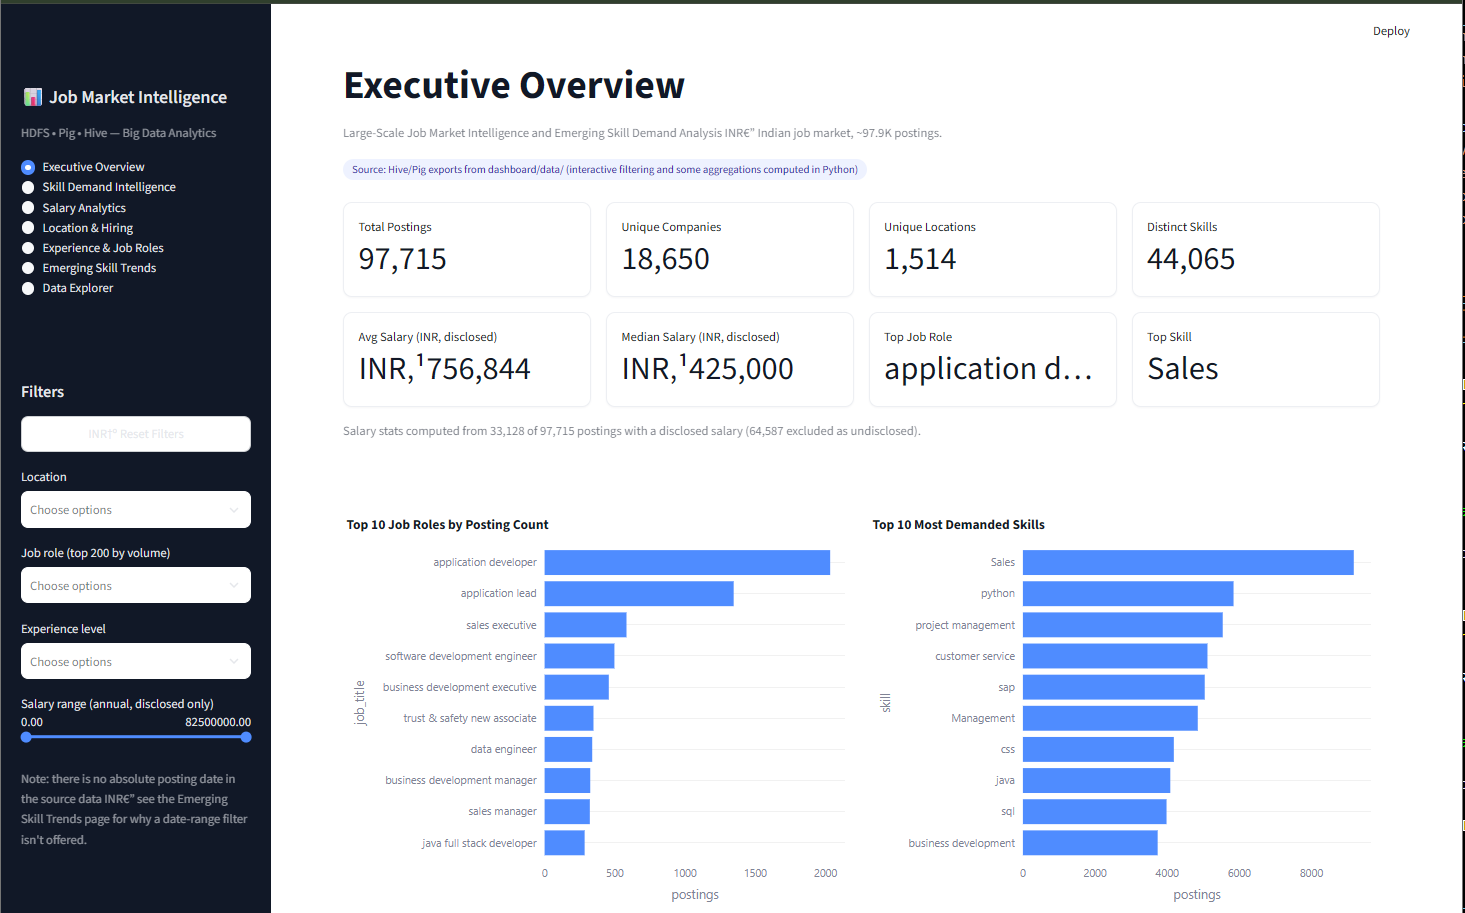
\includegraphics[width=0.48\textwidth]{screenshots/executive-overview.png}}{\fbox{\parbox[c][5cm][c]{0.45\textwidth}{\centering Executive Overview\\(screenshot not found)}}}\hfill
\IfFileExists{screenshots/skill-demand.png}{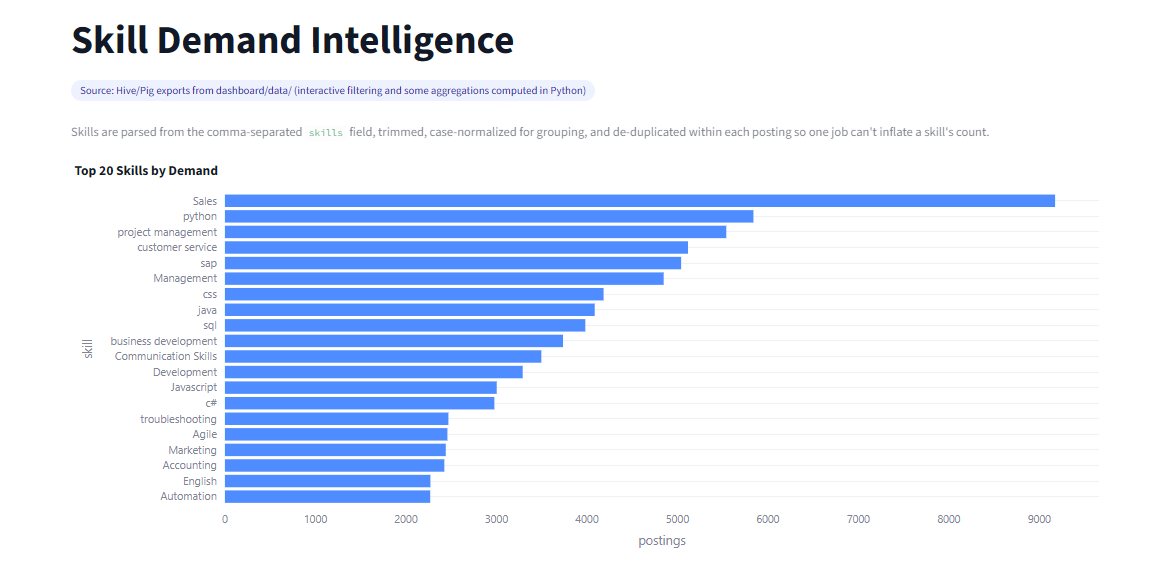
\includegraphics[width=0.48\textwidth]{screenshots/skill-demand.png}}{\fbox{\parbox[c][5cm][c]{0.45\textwidth}{\centering Skill Demand Intelligence\\(screenshot not found)}}}
\caption{Streamlit dashboard: Executive Overview (left) and Skill Demand Intelligence (right).}
\label{fig:dashboard_views}
\end{figure}

% =====================================================
%                 8. PHASE II / SDVI
% =====================================================
\section{Audit of Phase II and the Velocity Framework}

\subsection{Forensic Audit of Repository Artifacts}
Earlier drafts described an empirical Phase~II that processed 10,000 dated LinkedIn technology postings from January to June 2024 to compute a \textit{Skill Demand Velocity Index (SDVI)}. A systematic audit of the codebase, Git history, and HDFS cluster found:
\begin{itemize}
  \item \textbf{Filesystem and Git:} no files named \code{linkedin_postings.csv}, \code{clean_and_extract.pig}, \code{sdvi_query.hql}, \code{sdvi_results.json}, or \code{index.html} exist in the working tree or in any historical commit.
  \item \textbf{HDFS metadata:} offline analysis of NameNode metadata (\code{fsimage_0000000000000029319}) confirmed that the documented directory \code{/user/ashmi_sn/jobmarket/raw/} was never created.
\end{itemize}

In keeping with academic integrity, Phase~II is classified as \textbf{unimplemented and unverified} as an empirical pipeline. The proposed methodology is nevertheless a useful conceptual model and is evaluated theoretically below.

\subsection{Mathematical Formulation of SDVI}
The proposed index is defined as
\begin{equation}
\text{growth\_rate} = \frac{\text{Mentions}_t - \text{Mentions}_{t-1}}{\text{Mentions}_{t-1}}
\label{eq:growth}
\end{equation}
\begin{equation}
\text{SDVI} = \text{growth\_rate} \times \ln(1 + \text{Mentions}_t)
\label{eq:sdvi}
\end{equation}

\textbf{Validation of the stated examples:}
\begin{itemize}
  \item \textit{Low-volume jump ($2 \rightarrow 4$ mentions):} $\text{growth\_rate} = (4-2)/2 = 1.0$, so $\text{SDVI} = 1.0 \times \ln 5 \approx \mathbf{1.61}$.
  \item \textit{High-volume jump ($100 \rightarrow 150$ mentions):} $\text{growth\_rate} = 0.5$, so $\text{SDVI} = 0.5 \times \ln 151 \approx \mathbf{2.51}$.
\end{itemize}
The logarithmic factor curbs percentage inflation for low-frequency niche skills while preserving momentum signals for high-volume tools.

\subsection{Critique of the Quadrant Boundary Rules}
The original report classified skills into four quadrants using $\text{growth\_rate}$ and $\text{median(SDVI)}$ (Table~\ref{tab:quadrants}).

\begin{table}[htbp]
\centering
\small
\begin{tabular}{@{}ll@{}}
\toprule
\textbf{Quadrant} & \textbf{Proposed Rule} \\
\midrule
Emerging & $\text{growth\_rate} > 0$ and $\text{SDVI} > \text{median(SDVI)}$ \\
Established Growth & $\text{growth\_rate} > 0$ and $\text{SDVI} \le \text{median(SDVI)}$ \\
Stable Core & $\text{growth\_rate} \le 0$ and $\text{SDVI} > \text{median(SDVI)}$ \\
Declining & $\text{growth\_rate} \le 0$ and $\text{SDVI} \le \text{median(SDVI)}$ \\
\bottomrule
\end{tabular}
\caption{Original SDVI quadrant decision rules.}
\label{tab:quadrants}
\end{table}

\textbf{The Stable Core rule is unsatisfiable.}
\begin{enumerate}
  \item Since $\text{Mentions}_t \ge 0$, the factor $\ln(1 + \text{Mentions}_t)$ is non-negative.
  \item Hence the sign of $\text{SDVI}$ equals the sign of $\text{growth\_rate}$, so $\text{growth\_rate} \le 0 \implies \text{SDVI} \le 0$.
  \item In an active, growing market the median SDVI across skills is positive.
  \item Therefore, for any skill with $\text{growth\_rate} \le 0$, we have $\text{SDVI} \le 0 < \text{median(SDVI)}$.
  \item The rule $\text{growth\_rate} \le 0 \land \text{SDVI} > \text{median}$ can never hold.
  \item A ubiquitous incumbent (e.g., Python with 10,000 mentions and $0\%$ growth) gets $\text{SDVI} = 0 \le \text{median}$ and is wrongly labelled \textbf{``Declining''}.
\end{enumerate}

\subsection{Recommended Correction: Orthogonal Two-Dimensional Classification}
Volume and velocity should be placed on independent axes rather than multiplied together:
\begin{itemize}
  \item \textbf{Momentum (Y-axis):} $\Delta_t = (\text{Mentions}_t - \text{Mentions}_{t-1}) / (\text{Mentions}_{t-1} + \epsilon)$, with $\epsilon = 1$ to avoid division by zero for newly emergent skills.
  \item \textbf{Presence (X-axis):} $V_t = \ln(1 + \text{Mentions}_t)$.
\end{itemize}

The corrected taxonomy is given in Table~\ref{tab:corrected}, where $\delta = 0.05$ is a 5\% stability band around zero growth.

\begin{table}[htbp]
\centering
\small
\begin{tabular}{@{}p{3.2cm}p{5.8cm}p{4.6cm}@{}}
\toprule
\textbf{Category} & \textbf{Boundary Rule} & \textbf{Interpretation} \\
\midrule
Emerging & $\Delta_t > +\delta$ and $V_t \le \text{Median}(V)$ & High growth, early adoption \\
Established Growth & $\Delta_t > +\delta$ and $V_t > \text{Median}(V)$ & High growth, high enterprise adoption \\
Stable Core & $|\Delta_t| \le \delta$ and $V_t > \text{Median}(V)$ & Flat growth, dominant incumbent \\
Declining / Niche & $\Delta_t < -\delta$, or $|\Delta_t| \le \delta$ and $V_t \le \text{Median}(V)$ & Cooling demand or obsolete technology \\
\bottomrule
\end{tabular}
\caption{Corrected orthogonal classification of skill momentum.}
\label{tab:corrected}
\end{table}

% =====================================================
%                 9. LIMITATIONS
% =====================================================
\section{Data Integrity and Limitations}
\begin{itemize}
  \item \textbf{Currency isolation:} INR and USD are strictly segregated. Undisclosed compensation is handled by null propagation rather than zero-imputation, avoiding artificial deflation of salary means.
  \item \textbf{Text normalisation boundaries:} Task~2 applies lowercasing and whitespace trimming only. It does not merge semantic synonyms (e.g., \code{"sde"} and \code{"software development engineer"}). A canonical ontology mapping layer is recommended for production.
  \item \textbf{No longitudinal dates:} the dataset is a single scrape with relative recency strings and cannot support multi-year growth curves without fabricating dates.
  \item \textbf{Decoupled dashboard:} the Streamlit application runs independently of live cluster services. Production use requires scheduled refreshes of exported datasets (e.g., Apache Oozie or Airflow).
\end{itemize}

% =====================================================
%                 10. CONCLUSION
% =====================================================
\section{Conclusion and Future Work}

\subsection{Conclusion}
This project designed, implemented, and audited a scalable batch-processing Big Data pipeline over 97,929 Indian job postings. HDFS provides fault-tolerant storage, Apache Pig performs MapReduce-based transformation and tokenisation, and Apache Hive delivers structured SQL analytics through \code{OpenCSVSerde}, so the system processes data end to end without single-node memory bottlenecks.

The findings show that enterprise software roles (\textit{application developer}) and foundational skills (\textit{Python}, \textit{SAP}, \textit{Java}, \textit{SQL}) dominate recruitment volume, with over 38.5\% of openings concentrated in Bengaluru, Hyderabad, and Pune. Disclosed compensation is strongly right-skewed, with data engineering and architecture roles leading technology pay. Earlier reporting discrepancies were resolved as CSV export formatting artifacts. Finally, the limits of snapshot data were addressed through a mathematical evaluation of the Skill Demand Velocity Index.

\subsection{Future Work}
\begin{enumerate}
  \item \textbf{Longitudinal multi-scrape ingestion:} scheduled weekly scrapers writing to dated HDFS directories (e.g., \code{/jobmarket/raw/year=YYYY/month=MM/}) to enable true time-series analytics in Hive.
  \item \textbf{Ontological synonym mapping:} a domain-specific labour-market ontology to canonicalise spelling variants and synonymous role titles into standard occupation codes.
  \item \textbf{Orthogonal SDVI:} implement the corrected two-dimensional taxonomy in HiveQL using partitioned \code{LAG()} window queries over multi-month data.
  \item \textbf{Pipeline orchestration:} replace manual bash runners with a workflow orchestrator such as Apache Airflow covering cluster startup, ingestion, Pig execution, and dashboard export refresh.
\end{enumerate}

% =====================================================
%                 REFERENCES
% =====================================================
\begin{thebibliography}{99}
\addcontentsline{toc}{section}{References}

\bibitem{dean2004mapreduce}
J.~Dean and S.~Ghemawat, ``MapReduce: Simplified data processing on large clusters,'' in \textit{Proc. 6th Symposium on Operating Systems Design and Implementation (OSDI)}, 2004, pp. 137--150.

\bibitem{shvachko2010hdfs}
K.~Shvachko, H.~Kuang, S.~Radia, and R.~Chansler, ``The Hadoop Distributed File System,'' in \textit{Proc. IEEE 26th Symposium on Mass Storage Systems and Technologies (MSST)}, 2010, pp. 1--10.

\bibitem{olston2008pig}
C.~Olston, B.~Reed, U.~Srivastava, R.~Kumar, and A.~Tomkins, ``Pig Latin: A not-so-foreign language for data processing,'' in \textit{Proc. ACM SIGMOD International Conference on Management of Data}, 2008, pp. 1099--1110.

\bibitem{thusoo2009hive}
A.~Thusoo, J.~S.~Sarma, N.~Jain, Z.~Shao, P.~Chakka, S.~Anthony, H.~Liu, P.~Wyckoff, and R.~Murthy, ``Hive: A warehousing solution over a map-reduce framework,'' \textit{Proc. VLDB Endowment}, vol.~2, no.~2, pp. 1626--1629, 2009.

\bibitem{white2015hadoop}
T.~White, \textit{Hadoop: The Definitive Guide}, 4th~ed. Sebastopol, CA: O'Reilly Media, 2015.

\bibitem{khaouja2021survey}
S.~Khaouja, I.~Kassou, and M.~Ghogho, ``A survey on skill identification from online job ads,'' \textit{IEEE Access}, vol.~9, pp. 118434--118454, 2021.

\bibitem{djumalieva2018taxonomy}
J.~Djumalieva and C.~Sleeman, ``An open and data-driven taxonomy of skills extracted from online job adverts,'' Nesta Working Paper No.~18/03, 2018.

\bibitem{jobmarketrepo}
N.~Medhashree, A.~S.~N, and D.~Tudu, ``Job market intelligence and emerging skill demand analysis,'' GitHub repository, 2026. [Online]. Available: \url{https://github.com/medhashree05/JOB_MARKET_ANALYSIS}
\end{thebibliography}

\end{document}
